\documentclass[12pt,a4paper,oneside]{report}             % Single-side

\usepackage{amsmath}
\usepackage{amssymb}
\usepackage{anysize}


% EZZEL NEM JÓ
%\usepackage[thmmarks]{ntheorem}

% EZZEL JÓ
\usepackage{ntheorem}

%--------------------------------------------------------------------------------------
% Page layout setup
%--------------------------------------------------------------------------------------
% we need to redefine the pagestyle plain
% another possibility is to use the body of this command without \fancypagestyle
% and use \pagestyle{fancy} but in that case the special pages
% (like the ToC, the References, and the Chapter pages)remain in plane style

\pagestyle{plain} % ellentmond a pagestyle fancy-nek
\setlength{\parindent}{0pt} % áttekinthetőbb, angol nyelvű dokumentumokban jellemző
\setlength{\parskip}{9pt plus 3pt minus 3pt} % áttekinthetőbb, angol nyelvű dokumentumokban jellemző
\marginsize{35mm}{25mm}{15mm}{15mm} % anysize package - VÉGLEGESHEZ


\begin{document}
\begin{equation} \label{eq_hofelvetel}
\dot Q_{fel} = c ~ \dot{m} ~ \Delta t
\end{equation}


\begin{equation} \label{eq_holeadas2}
\begin{aligned}
\dot Q_{le} = k_e ~ A_e ~ \left( \frac{t_s+t_r}{2}-t_i\right) = k_e ~ A_e ~ \left( \frac{t_s+(t_s-\Delta t)}{2}-t_i-t_{drop}\right)
\end{aligned}
\end{equation}

Ahol felhasználtuk azt is, hogy $t_r = t_s-\Delta t$, majd $\Delta t$ helyére beírhatjuk a (\ref{eq_hofelvetel})  átrendezett alakját:
\begin{equation} \label{eq_hofelvetel2}
~~\Delta t = \frac{\dot Q_{fel}}{c ~ \dot{m}}
\end{equation}

Beírva (\ref{eq_holeadas2})-ba (\ref{eq_hofelvetel2})-t:

A \ref{f}. figure

\begin{figure}
	\centering
	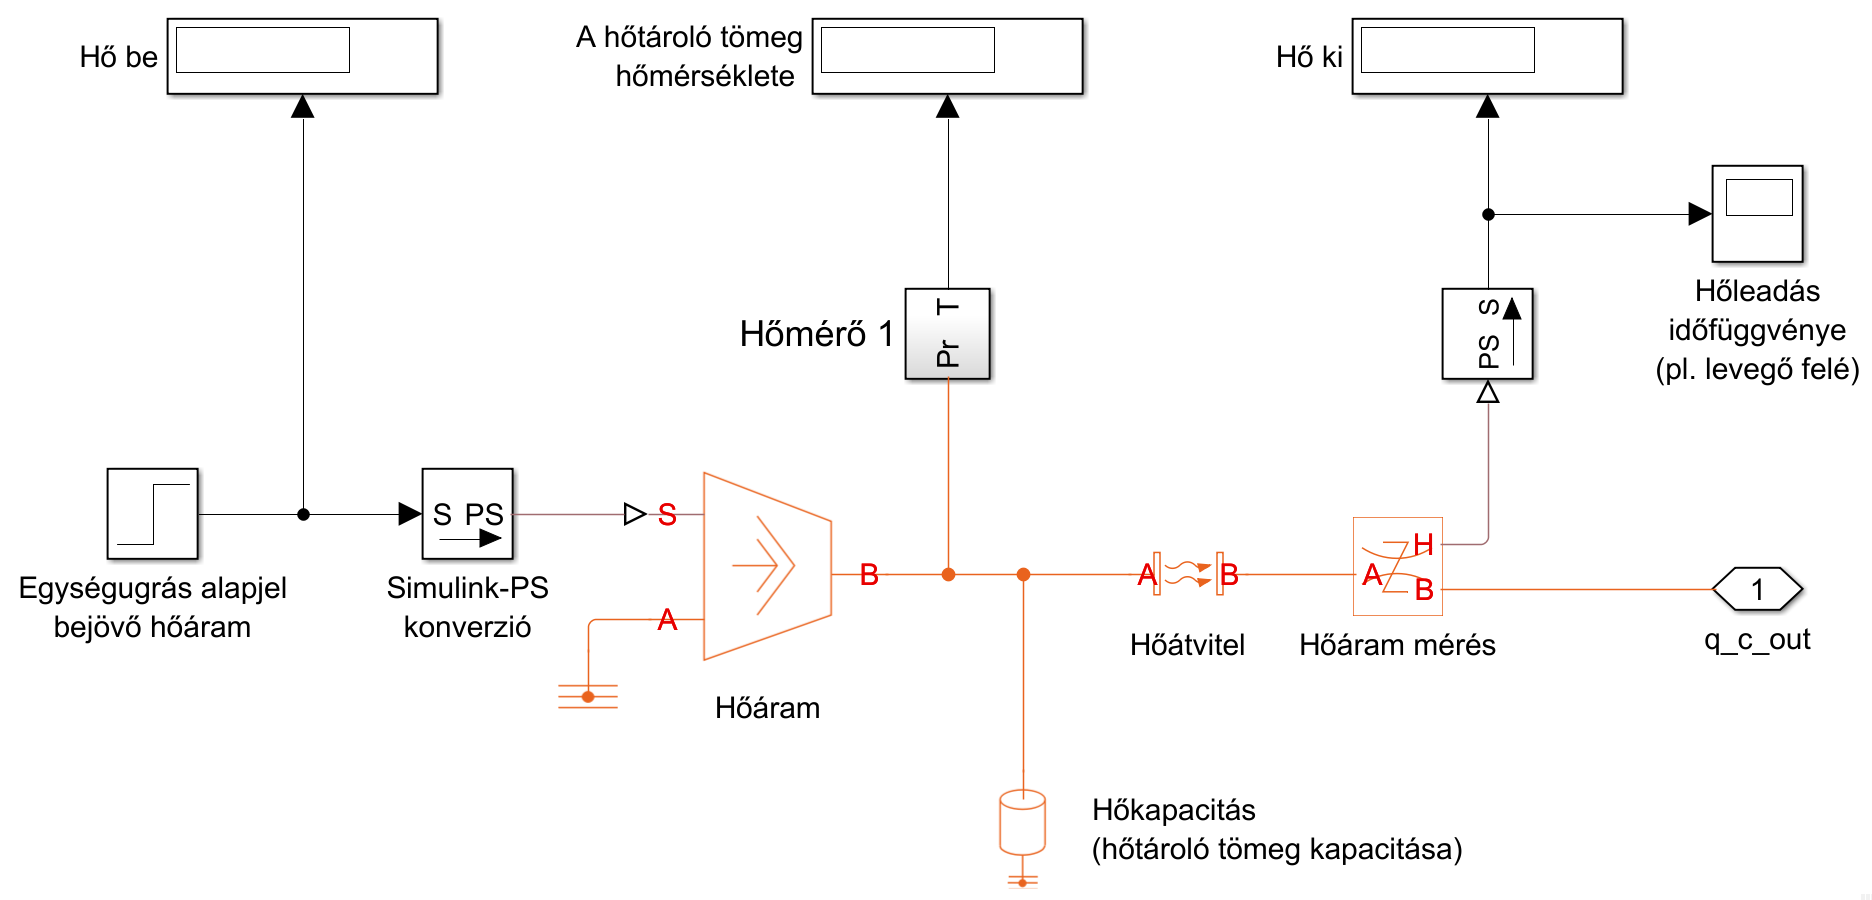
\includegraphics[width=\textwidth]{figures/SimscapeGeneral}
	\caption{Simscape termikus blokkok a Simulinkben}
	\label{f}
\end{figure}

A \ref{f}. figure
\end{document}
